%% Estructura principal para un reporte de Trabajos intersemanales CIRCAE %%
\documentclass[a4paper]{IEEEtran} %tamaño del papel y el tipo de transcripción que será IEEE
\usepackage[utf8]{inputenc} %el tipo de codificación que incluye símbolos como la tilde
\usepackage[spanish]{babel} % hacemos que nuestro documentación vaya en español
\usepackage{cite} % citas bibliográficas
\usepackage{graphicx} %gráficos, usaremos solo .jpg o .png con estándares que ya veremos
\usepackage{subfigure} %usar subfiguras
\usepackage{url} %agregar direcciones url
\usepackage{amsmath} %expresiones matemáticas
\newtheorem{teor}{Teorema}[section] %definimos la enumeración de Teoremas usando la etiqueta \begin{teor} ... \end{teor} para los ejemplos, podemos darle etiquetas para referenciarlas a lo largo del texto
\newtheorem{ejem}{Ejemplo}[section] %definimos la enumeración de Ejemplos usando la etiqueta \begin{ejem} ... \end{ejem} para los ejemplos, podemos darle etiquetas para referenciarlas a lo largo del texto
\newtheorem{exper}{Experimento}[section] %definimos la enumeración de Ejemplos usando la etiqueta \begin{exper} ... \end{exper} para los Experimentos, podemos darle etiquetas para referenciarlas a lo largo del texto
\usepackage{setspace} %LA usamos para asignar el interlineado
%%%%%%% settings para incluir codigo fuente en cualquier lenguaje
\usepackage{listings} %comenzamos la configuración de nuestras lineas de codigo que se incluirá de ser necesario en el documento
\usepackage[usenames]{color} %seteamos el uso de nombre y color
\definecolor{gray97}{gray}{.97}%definimos nombre y color
\definecolor{gray75}{gray}{.75}%definimos nombre y color
\definecolor{gray45}{gray}{.45}%definimos nombre y color
\definecolor{azul1}{RGB}{141,198,163}%definimos nombre y color
\definecolor{azul2}{RGB}{24,107,122}%definimos nombre y color
\definecolor{verde1}{RGB}{44,186,34}%definimos nombre y color
\usepackage{textcomp}
\lstset{
		frame=Ltb,
		framerule=1pt,
		framextopmargin=3pt,
		framexbottommargin=3pt,
		framexleftmargin=0.4cm,
		framesep=0pt,
		rulesep=.4pt,
		backgroundcolor=\color{gray97},
		rulesepcolor=,
        tabsize=4,
        rulecolor=\color{azul1},
        basicstyle=\scriptsize\ttfamily,
        upquote=true,
        aboveskip={1.5\baselineskip},
        columns=fixed,
        showstringspaces=false,
        extendedchars=true,
        breaklines=true,
        prebreak = \raisebox{0ex}[0ex][0ex]{\ensuremath{\hookleftarrow}},
        showtabs=false,
        showspaces=false,
        showstringspaces=false,
        identifierstyle=\ttfamily,
        keywordstyle=\color[rgb]{0,0,1},
        commentstyle=\color[rgb]{0.133,0.545,0.133},
        stringstyle=\color[rgb]{0.627,0.126,0.941},
        keywordstyle=\bfseries,
        %
		numbers=left,
		numbersep=15pt,
		numberstyle=\tiny,
		numberfirstline = false,
		breaklines=true,
		}
\usepackage{graphicx}
\usepackage[colorinlistoftodos]{todonotes}
%%%%%%%
\providecommand{\keywords}[1]{\textbf{\textit{Términos Clave---}} #1}

\begin{document}
\spacing{0.9} %definimos un interlineado de 0.9 para todo el documento

\title{Nomre del Proyecto en Puestión}
\author{NombreA1 ApellidoA1 ApellidoA2, Miembro, CIRCAE, NombreB1 ApellidoB1 ApellidoB2, Miembro, CIRCAE
\thanks{Este primer párrafo puede contener auspiciadores u organizaciones que colaboraron con la realización de esta parte del proyecto y mencionar de manera expecífica que papel puntual tuvieron en el proceso... "This work was supported in part by the U.S. Department of Commerce under Grant BS123456."}
\thanks{Los siguientes párrafos pueden contebner datos específicos de los autores del proyecto, por ejemplo "F. A. Author is with the National Institute of Standards and Technology, Boulder, CO 80305 USA (e-mail: author\@ boulder.nist.gov)"}
\thanks{NombreA1 ApellidoA1 ApellidoA2, was with Rice University, Houston, TX 77005 USA. He is now with the Department of Physics, Colorado State University, Fort Collins, CO 80523 USA (e-mail: author\@ lamar.colostate.edu).}
\thanks{NombreB1 ApellidoB1 ApellidoB2 is with the Electrical Engineering Department, University of Colorado, Boulder, CO 80309 USA, on leave from the National Research Institute for Metals, Tsukuba, Jaan (e-mail: author\@ nrim.go.jp).}}

\markboth{CIRCAE INFORME 201901-07-31-G1-P3-005}{} % Codigo del informe que corresponde a: semestre | mes | dia | numero de grupo con la G antepuesta | numero de proyecto con la P antepuesta | número de informe
\maketitle


\begin{abstract}
MicroMouse es un dispositivo en el que se aplica principios de ciencias de la computación, principios ópticos, mecánicos, electrónicos y la integración de tecnologías de software y hardware \cite{libro1} . Lo que se pretende cubrir es la solución de un laberinto usando algoritmos de reconocimiento, almacenamiento, solución y retroalimentación con condiciones iniciales constantes en el tiempo.\\

\keywords{\textbf{Introducimos nuestros términos clave en orden alfabetico, separado por comas. Para una lista de sugerencias de palabras o términos clave visitar \underline{http://www.ieee.org/organizations/pubs/ani\_ prod/keywrd98.txt}}}
\end{abstract}




\section{Problema}
\label{problema} %Tambien se puede poner etiquetas a secciones, subsecciones, subsubsecciones
    
El problema será planteado con un pequeño preambulo y luego enumerado con items de la siguiente manera:
    
    \begin{itemize}
    	\item Este es la primera parte del problema
    	\item Segunda parte del prblema, y se puede saltar al siguiente sin necesidad de agregar barras ivertidas %estos --> \\
		\item Tercer item tambien importante, y así se púede agregar más items al problema
	\end{itemize}
	
	Otra manera de agregar partes del problema es enfatizando algunas palabras, usándolo de la siguiente manera:
	
	\begin{itemize}
		\item \textbf{Interferencia} que nos lleva a la descripción del problema relacionado con interferencia.
		\item \textbf{Ahorro energetico} en los circuitos en la fase de prototipado, que por lo general tienen un alto consumo energético.
	\end{itemize}

El uso de los items no es necesario si se tiene bien definido solo un punto, o dos, los cuales pueden ser abordados en un solo párrafo, o en más de ser necesarios, para ello siempre haremos uso de las dos barras invertidas\\ % estos --> \\
Como se podrán dar cuenta, si incluimos estas dos barras, y solo saltamos un renglon, tendremos este resultado pero si incluimos las dos barras y luego saltamos un renglon como sigue \\

Tendremos este resultado, un párafo que tiene indentación, mientras que el anterior no lo tiene, tampoco tiene el espacio entre párrafo y párrafo extra.

De ser necesario se podría incluir algun gráfico pequeño, teniendo en cuenta que el máximo en ancho de imagen será de $8.5cm$ como se muestra en la figura \eqref{img1}, tomar este dato con cautela, ya que gráficos como una captura de pantalla no podrán mostrar toda su informacion en 8.5cm de ancho.

\begin{figure} %Comenzar la figura
    \centering %hacemos que la imagen en cuestion esté centrada, si guera de 5 o 6 cm, esta se vea bien
        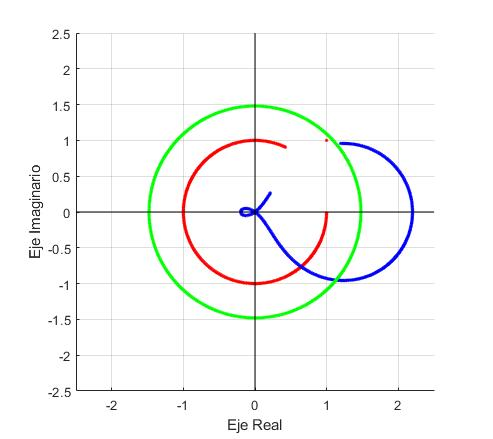
\includegraphics[width=8.5cm]{imagenes/img1} %incluimos la imagen con una característica especial: la medida definida en centímetros e incluimos la ruta de imagen sin especificar la extensión de la imagen (solo usaremos .png y .jpg)
        \caption{Un gráfico de Matlab} %La descripción de la imagen, ser concisos
        \label{img1} %La etiqueta usada para poder referenciarla desde cualquier parte del texto como se hizo con /eqref{img1}
\end{figure} %finalizamos la figura

\section{Objetivos}

Descripcion sencilla con los mismos parámetros de ''Problemas''  en \eqref{problema} %Ojo, para las comillas, usar las comillas simples 'para este texto', o dos veces las comillas simples ''para usar las comillas dobles'',

\section{Procedimiento}
\label{procedimiento}

El planteamiento debe extar expresado en un lenguaje claro, no redundante y bien detallado. Citando libros, artículos (referencias externas en general como \cite{libro1} , o citando carios libros a la vez \cite{libro2, libro2, libro3}), tambien haciendo referencia a teoremas, ejemplos, ecuaciones

\begin{teor}
\rm
\label{fhfthfy_}
El \textbf{Teorema de Feynman} relaciona el derivado de la energía total con respecto a un parámetro, al valor de la expectativa del derivado del hamiltoniano con respecto a ese mismo parámetro. Su aplicación más común está en el cálculo de fuerzas en moléculas (con los parámetros que son las posiciones de los núcleos) donde declara que una vez que la distribución espacial de los electrones se ha determinado solucionando la ecuación de Schrödinger, todas las fuerzas en el sistema se pueden calcular usando conceptos de la electrostática clásica.

\begin{equation}
\bigg\langle\frac {d\psi (\lambda)} {d\lambda } \left| \hat {H} _ {\lambda } \right| \psi (\lambda) \bigg\rangle + \langle\psi (\lambda)  |\hat {H} _ {\lambda } |\frac {d\psi (\lambda)} {d\lambda }\rangle + \bigg\langle\psi (\lambda) \bigg |\frac {d\hat {H} _ {\lambda}} {d\lambda } |\psi (\lambda) \bigg\rangle 
\end{equation}

\begin{eqnarray}
 \frac1{t - z} & = & \frac1{t - a - (z - a)} \\
 & = & \frac1{t - a}
  \left( \frac1{1 - \frac{z - a}{t - a}} \right) \\
 & = & \frac1{t - a}
  \left[ \sum_{i=0}^n \left( \frac{z - a}{t - a} \right)^n
  + \frac{\left( \frac{z - a}{t - a} \right)^{n+1}}
  {1 + \frac{z - a}{t - a}} \right]
\end{eqnarray}

\end{teor}

\subsection{Types of Graphics}
The following list outlines the different types of graphics published in 
IEEE journals. They are categorized based on their construction, and use of 
color/shades of gray:

\begin{figure}%
\centering
\subfigure[]{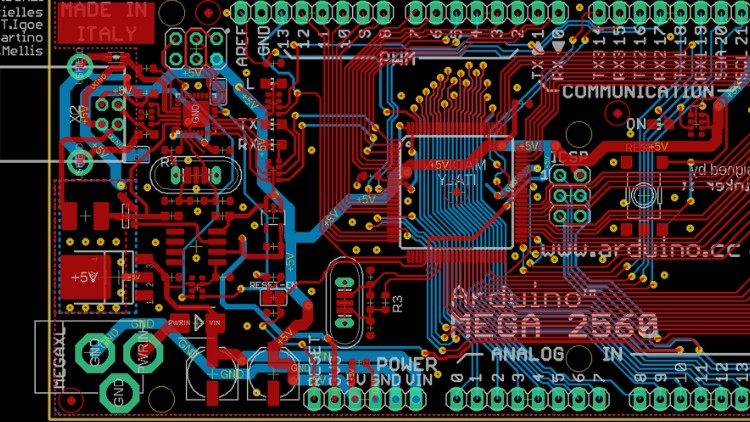
\includegraphics[width=8cm]{imagenes/img2} \label{subfiguraA}}
\subfigure[]{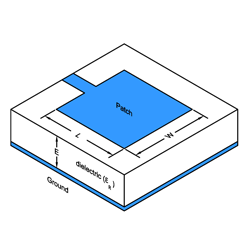
\includegraphics[width=4cm]{imagenes/img3} \label{subfiguraB}}
\subfigure[]{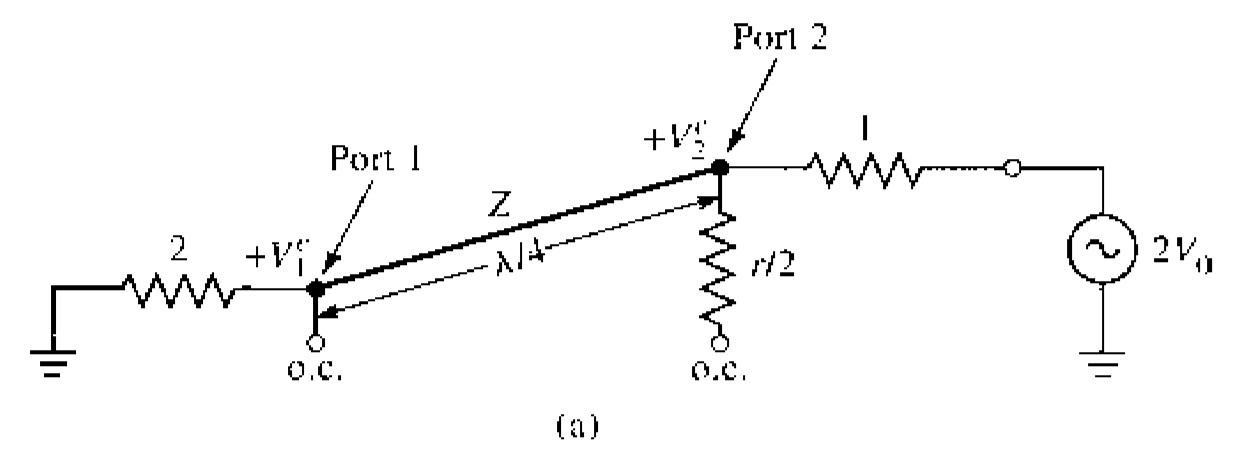
\includegraphics[width=4cm]{imagenes/img4} \label{subfiguraC}}
\caption{Tenemos tres subfiguras, la subfigura \ref{subfiguraA}, tambien tenemos la \ref{subfiguraB} y la \ref{subfiguraC}}
\label{3figs}
\end{figure}

\subsubsection{Color/Grayscale figures}
{Figures that are meant to appear in color, or shades of black/gray. Such 
figures may include photographs, illustrations, multicolor graphs, and 
flowcharts.}



\subsubsection{Line Art figures}
{Figures that are composed of only black lines and shapes. These figures 
should have no shades or half-tones of gray, only black and white.}

\begin{figure}
    \centering
        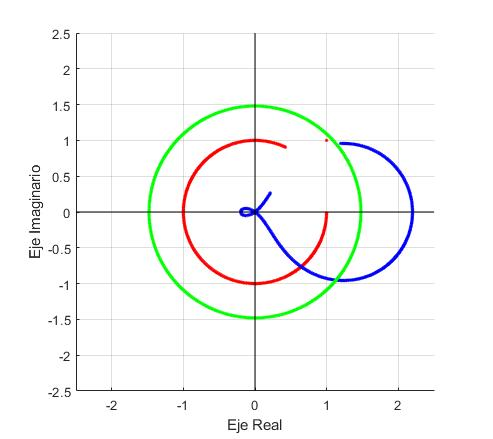
\includegraphics[width=8cm]{imagenes/img1}
        \caption{A gull}
        \label{fig:gull}
\end{figure}

\subsubsection{Author photos}
{Head and shoulders shots of authors that appear at the end of our papers. }

\subsection{Lineas de código}



\noindent
Ahora compila usando \texttt{gcc}:



\subsubsection{Tables}
{Data charts which are typically black and white, but sometimes include 
color.}

\begin{table}
\caption{Units for Magnetic Properties}
\label{table}
\setlength{\tabcolsep}{3pt}
\begin{tabular}{|p{25pt}|p{75pt}|p{115pt}|}
\hline
Symbol& 
Quantity& 
Conversion from Gaussian and \par CGS EMU to SI $^{\mathrm{a}}$ \\
\hline
$\Phi $& 
magnetic flux& 
1 Mx $\to  10^{-8}$ Wb $= 10^{-8}$ V$\cdot $s \\
$B$& 
magnetic flux density, \par magnetic induction& 
1 G $\to  10^{-4}$ T $= 10^{-4}$ Wb/m$^{2}$ \\
$H$& 
magnetic field strength& 
1 Oe $\to  10^{3}/(4\pi )$ A/m \\
$m$& 
magnetic moment& 
1 erg/G $=$ 1 emu \par $\to 10^{-3}$ A$\cdot $m$^{2} = 10^{-3}$ J/T \\
$M$& 
magnetization& 
1 erg/(G$\cdot $cm$^{3}) =$ 1 emu/cm$^{3}$ \par $\to 10^{3}$ A/m \\
4$\pi M$& 
magnetization& 
1 G $\to  10^{3}/(4\pi )$ A/m \\
$\sigma $& 
specific magnetization& 
1 erg/(G$\cdot $g) $=$ 1 emu/g $\to $ 1 A$\cdot $m$^{2}$/kg \\
$j$& 
magnetic dipole \par moment& 
1 erg/G $=$ 1 emu \par $\to 4\pi \times  10^{-10}$ Wb$\cdot $m \\
$J$& 
magnetic polarization& 
1 erg/(G$\cdot $cm$^{3}) =$ 1 emu/cm$^{3}$ \par $\to 4\pi \times  10^{-4}$ T \\
$\chi , \kappa $& 
susceptibility& 
1 $\to  4\pi $ \\
$\chi_{\rho }$& 
mass susceptibility& 
1 cm$^{3}$/g $\to  4\pi \times  10^{-3}$ m$^{3}$/kg \\
$\mu $& 
permeability& 
1 $\to  4\pi \times  10^{-7}$ H/m \par $= 4\pi \times  10^{-7}$ Wb/(A$\cdot $m) \\
$\mu_{r}$& 
relative permeability& 
$\mu \to \mu_{r}$ \\
$w, W$& 
energy density& 
1 erg/cm$^{3} \to  10^{-1}$ J/m$^{3}$ \\
$N, D$& 
demagnetizing factor& 
1 $\to  1/(4\pi )$ \\
\hline
\multicolumn{3}{p{251pt}}{Vertical lines are optional in tables. Statements that serve as captions for 
the entire table do not need footnote letters. }\\
\multicolumn{3}{p{251pt}}{$^{\mathrm{a}}$Gaussian units are the same as cg emu for magnetostatics; Mx 
$=$ maxwell, G $=$ gauss, Oe $=$ oersted; Wb $=$ weber, V $=$ volt, s $=$ 
second, T $=$ tesla, m $=$ meter, A $=$ ampere, J $=$ joule, kg $=$ 
kilogram, H $=$ henry.}
\end{tabular}
\label{tab1}
\end{table}

\subsection{Multipart figures}
Figures compiled of more than one sub-figure presented side-by-side, or 
stacked. If a multipart figure is made up of multiple figure
types (one part is lineart, and another is grayscale or color) the figure 
should meet the stricter guidelines.

\subsection{File Formats For Graphics}\label{formats}
Format and save your graphics using a suitable graphics processing program 
that will allow you to create the images as PostScript (PS), Encapsulated 
PostScript (.EPS), Tagged Image File Format (.TIFF), Portable Document 
Format (.PDF), Portable Network Graphics (.PNG), or Metapost (.MPS), sizes them, and adjusts 
the resolution settings. When 
submitting your final paper, your graphics should all be submitted 
individually in one of these formats along with the manuscript.

\begin{equation}
\frac{\partial u}{\partial t}
   = h^2 \left( \frac{\partial^2 u}{\partial x^2}
      + \frac{\partial^2 u}{\partial y^2}
      + \frac{\partial^2 u}{\partial z^2} \right)
\end{equation}


\section{Conclusiones}
A conclusion section is not required. Although a conclusion may review the 
main points of the paper, do not replicate the abstract as the conclusion. A 
conclusion might elaborate on the importance of the work or suggest 
applications and extensions. 

\lstinputlisting[language=Octave]{codigo/graf1.m}


%La bibliografía:
\bibliographystyle{ieeetr}
\bibliography{bibliografia}

\end{document}